%%%%%%%%%%%%%%%%%%%%%%%%%%%%%%%%%%%%%%%%%%%%%%%%%%%%%%%%%%%%%%%%%%%%%%%%%%%%%%%
% A clean template for an academic CV. This is a short summary version.
%
% Uses tabularx to create two column entries (date and job/edu/citation).
% Defines commands to make adding entries simpler.
%
%%%%%%%%%%%%%%%%%%%%%%%%%%%%%%%%%%%%%%%%%%%%%%%%%%%%%%%%%%%%%%%%%%%%%%%%%%%%%%%

\documentclass[9pt,a4paper]{article}

% === Load packages ===

% Insert image file
\usepackage[dvipdfmx]{graphicx}

% Full Unicode support for non-ASCII characters
\usepackage[utf8]{inputenc}
\usepackage[english]{babel}
\usepackage[TU]{fontenc}

% Set main fonts
\usepackage[sfdefault]{atkinson}
\usepackage[ttdefault]{sourcecodepro}
% \usepackage[sfdefault]{FiraSans}

% For Japanese characters
\usepackage{xeCJK}
\setCJKmainfont{Noto Sans CJK JP}  % for Linux
% \setCJKmainfont{Noto Sans JP}  % for MacOS

% Icon fonts
\usepackage{fontawesome5}
\usepackage{academicons}
\newcommand{\faDblp}{\hspace{-0.20em}\raisebox{-0.25em}{
\includegraphics[height=1.1em]{./fig/dblp.png}}\hspace{-0.1em}}

% Disable hyphenation
% \usepackage[none]{hyphenat}

\usepackage{ifthen}

% Control the font size
\usepackage{anyfontsize}

% For fancy and multipage tables
\usepackage{tabularx}
\usepackage{ltablex}

% For new environments
\usepackage{environ}

% Manage dates and times
\usepackage{datetime}

% Set the page margins
\usepackage{geometry}

% To get the total page numbers (\pageref{LastPage})
\usepackage{zref-totpages}

% Control spacing in enumerates
\usepackage{enumitem}

% Use custom colors
\usepackage[usenames,dvipsnames]{xcolor}

% Configure section titles
\usepackage{titlesec}

% Fancy header configuration
\usepackage{fancyhdr}

% Control PDF metadata and links
\usepackage[colorlinks=true]{hyperref}

% Underline
\usepackage{lib/culine}
\usepackage[normalem]{ulem}
\usepackage{soul}

\usepackage{tikz}
\usepackage{fontspec} % if using lualatex or xelatex
\usetikzlibrary{calc}
\usepackage{expl3}

% Useful aliases
\newcommand{\OU}{The University of Osaka}

% Identifying information
\newcommand{\Title}{Curriculum Vit\ae\ Summary}
\newcommand{\FirstName}{Naoki}
\newcommand{\LastName}{Chihara}
\newcommand{\MyName}{\FirstName\ \LastName}
\newcommand{\Me}{\smartunderline{\FirstName\ \LastName}}  % For citations
\newcommand{\Email}{naoki88[at]sanken.osaka-u.ac.jp}
\newcommand{\PersonalWebsite}{c-naoki.vercel.app}
\newcommand{\LabWebsite}{www.dm.sanken.osaka-u.ac.jp}
\newcommand{\ORCID}{0009-0005-7061-8214}
\newcommand{\GitHubProfile}{C-Naoki}
\newcommand{\Linkedin}{c-naoki}
\newcommand{\Gscholar}{pq2b3jQAAAAJ}
\newcommand{\Twitter}{c_naoki13}

% Names
\newcommand{\Prof}[1]{Prof.\! #1}
\newcommand{\YSakurai}{Yasushi Sakurai}
\newcommand{\YMatsubara}{Yasuko Matsubara}
\newcommand{\RFujiwara}{Ren Fujiwara}
\newcommand{\MOnizuka}{Makoto Onizuka}

% URLs
\newcommand{\YSakuraiURL}{https://www.dm.sanken.osaka-u.ac.jp/~yasushi/index-j.html}
\newcommand{\YMatsubaraURL}{https://www.dm.sanken.osaka-u.ac.jp/~yasuko/}
\newcommand{\MOnizukaURL}{http://www-bigdata.ist.osaka-u.ac.jp/professor/onizuka/onizuka_en.html}

% Language configuration
\def\lang{en}
\providecommand{\lang}{en}

\newcommand{\deflangvalue}[3]{%
  \ifthenelse{\equal{\lang}{en}}{%
    \expandafter\def\csname #1Value\endcsname{#2}%
  }{%
    \expandafter\def\csname #1Value\endcsname{#3}%
  }%
  \expandafter\def\csname #1\endcsname{\csname #1Value\endcsname}%
}

% common
\deflangvalue{OU}{The University of Osaka}{大阪大学}

% header
\deflangvalue{AddressLabel}{\textbf{Address}}{\textbf{住所}}
\deflangvalue{Affiliation}{SANKEN, \OU}{大阪大学 産業科学研究所}
\deflangvalue{Address}
{Mihogaoka 8-1, Ibaraki, Osaka 567-0047, Japan}
{565-0871 大阪府茨木市美穂ヶ丘 8-1}
\deflangvalue{EmailLabel}{\textbf{Email}}{\textbf{メール}}
\deflangvalue{EmailSuppl}
{please replace [at] with @}
{[at] を @ に置き換えてください}
\deflangvalue{UnivLabel}{\textbf{University}}{\textbf{大学}}
\deflangvalue{LabLabel}{\textbf{Laboratory}}{\textbf{研究室}}
\deflangvalue{WebsiteLabel}{\textbf{Website}}{\textbf{Webサイト}}
\deflangvalue{LastUpdatedLabel}{\textbf{Last Updated Date}}{\textbf{最終更新日}}

% education
\deflangvalue{Education}{Education}{学歴}
\deflangvalue{PhD}
{\textbf{Ph.D. in Information Science}, \OU}
{\textbf{博士(情報科学)}}
\deflangvalue{PhDDepartment}
{Department of Information Systems Engineering, Graduate School of Information Science and Technology}
{\OU\ 情報科学研究科\ 情報システム工学専攻}
\deflangvalue{ExpectedDate}
{Expected graduation date is March 2028}
{卒業予定日:2028年3月}
\deflangvalue{PhDSupervisor}
{Supervisor: \Prof{\YSakurai}}
{指導教員:櫻井保志教授}
\deflangvalue{MSc}
{\textbf{M.Sc.\! in Information Science}, \OU}
{\textbf{修士(情報科学)}}
\deflangvalue{MScDepartment}
{Department of Information Systems Engineering, Graduate School of Information Science and Technology}
{\OU\ 情報科学研究科\ 情報システム工学専攻}
\deflangvalue{MScThesis}
{Thesis: Stream Mining Time-evolving Causality for Time Series Forecasting}
{学位論文:時系列データストリームにおける将来予測のための時間変化する因果関係の抽出}
\deflangvalue{MScSupervisor}
{Supervisor: \Prof{\YSakurai}}
{指導教員:櫻井保志教授}
\deflangvalue{BSc}
{\textbf{B.Sc.\! in Engineering}, \OU}
{\textbf{学士(工学)}}
\deflangvalue{BScDepartment}
{Department of Electronic and Information Engineering, School of Engineering}
{\OU\ 工学部\ 電子情報工学科}
\deflangvalue{BScThesis}
{Thesis: Detection of Variable Celestial Objects using Machine Learning-based Periodic Analysis and Domain Knowledge}
{学位論文:機械学習による周期解析及びドメイン知識を活用した変動天体検出}
\deflangvalue{BScSupervisor}
{Supervisor: \Prof{\MOnizuka}}
{指導教員:鬼塚真教授}

% experience
\deflangvalue{Experience}{Experience}{職歴}
\deflangvalue{AIlabIntern}{AI Lab, CyberAgent}{株式会社サイバーエージェント AI Lab}
\deflangvalue{AIlabInternPosition}{Research Internship}{研究インターンシップ}
\deflangvalue{DC}{Japan Society for the Promotion of Science (JSPS)}{日本学術振興会 (JSPS)}
\deflangvalue{DCPosition}{Research Fellow DC1}{特別研究員 DC1}
\deflangvalue{SANKEN}{SANKEN, \OU}{\OU\ 産業科学研究所}
\deflangvalue{SANKENPosition}{Specially Appointed Researcher}{特任研究員}
\deflangvalue{TA}{School of Engineering, \OU}{工学部, 大阪大学}
\deflangvalue{TAPosition}{Teaching Assistant for ``Exercises in Mathematical Analysis''}{ティーチングアシスタント「数学解析演習」}
\deflangvalue{IST}{Graduate School of Information Science and Technology, \OU}{\OU\ 情報科学研究所}
\deflangvalue{ISTPosition}{Assistant in the detection of variable celestial objects}{変動天体の探索に関する補助}
\deflangvalue{Nagase}{Nagase Co., Ltd.}{株式会社ナガセ}
\deflangvalue{NagasePosition}{Digital Technology Engineer}{デジタル技術エンジニア}

% awards
\deflangvalue{Awards}{Awards}{受賞}
\deflangvalue{DEIM2025RunnerUp}
{DEIM2025 Best Paper Award Runner-up}
{DEIM2025 優秀論文賞}
\deflangvalue{OsakaUnivAward}
{Award of the Graduate School of Information Science and Technology of Osaka University}
{大阪大学情報科学研究科賞}
\deflangvalue{DEIM2025Presentation}
{DEIM2025 Student Presentation Award}
{DEIM2025 学生プレゼンテーション賞}
\deflangvalue{YamashitaAward}
{Information Processing Society of Japan (IPSJ) Yamashita SIG Research Award}
{情報処理学会\ 山下記念研究賞}
\deflangvalue{DEIM2024RunnerUp}
{DEIM2024 Best Paper Award Runner-up}
{DEIM2024 優秀論文賞}
\deflangvalue{HWIPScholarship}
{Osaka University Humanware Innovation Program Scholarship}
{ヒューマンウェアイノベーション博士課程プログラム}

% publications
\deflangvalue{Publications}{Publications}{研究業績}
\deflangvalue{Peerreviewed}{Peer-reviewed Publications}{査読付き論文}
\deflangvalue{NonPeerreviewed}{Non-refereed Publications}{査読なし論文}
\deflangvalue{Patents}{Patents}{特許}


\newcommand{\smartunderline}[1]{%
  \tikz[baseline=(X.base)]{
    \node[inner sep=0pt, outer sep=0pt] (X) {\strut #1};
    \draw[line width=0.5pt]
      ([yshift=0.6ex]X.south west) -- ([yshift=0.6ex]X.south east);
  }%
}

% Add semi-bold
\DeclareRobustCommand{\sbseries}{\fontseries{sb}\selectfont}
\DeclareTextFontCommand{\textsb}{\sbseries}

% Template configuration
%%%%%%%%%%%%%%%%%%%%%%%%%%%%%%%%%%%%%%%%%%%%%%%%%%%%%%%%%%%%%%%%%%%%%%%%%%%%%%%

\geometry{%
  margin=12.5mm,
  headsep=0mm,
  headheight=0mm,
  footskip=5mm,
  includehead=true,
  includefoot=true
}

% Custom colors
\definecolor{mediumgray}{gray}{0.5}
\definecolor{lightgray}{gray}{0.9}
\definecolor{mediumblue}{HTML}{2060c2}
\definecolor{lightblue}{HTML}{a0c3ff}
\definecolor{mediumred}{HTML}{ca8a03}

% No indentation
\setlength\parindent{0cm}

% Increase the line spacing
\renewcommand{\baselinestretch}{1.1}
% and the spacing between rows in tables
\renewcommand{\arraystretch}{1.25}

% Remove space between items in itemize and enumerate
\setlist{nosep}

% Set the spacing and format of sections
\titleformat{\section}
  % {\normalfont\Large\mdseries} % format
  {\fontsize{16}{19}\mdseries}
  {} % label
  {0pt} % separation (left separation for hang)
  {} % text before title
  [\titlerule] % text after title
\titlespacing*{\section}
  {0pt} % left pad
  {0.1cm} % before
  {0cm} % after

% Disable number of sections. Use this instead of "section*" so that the sections still
% appear as PDF bookmarks. Otherwise, would have to add the table of contents entries
% manually.
\makeatletter
\renewcommand{\@seccntformat}[1]{}
\makeatother

% Define a new environment to place all CV entries in a 2-column table.
% Left column are the dates, right column the entries.
\newcommand{\TablePad}{\vspace{-0.2cm}}
\NewEnviron{EntriesTableDuration}{
\TablePad
\begin{tabularx}{\textwidth}{@{}p{0.10\textwidth}@{\hspace{0.02\textwidth}}p{0.88\textwidth}@{}}
  \BODY
\end{tabularx}
\TablePad
}
\NewEnviron{EntriesTableYear}{
\TablePad
\begin{tabularx}{\textwidth}{@{}p{0.05\textwidth}@{\hspace{0.01\textwidth}}p{0.94\textwidth}@{}}
  \BODY
\end{tabularx}
\TablePad
}
\NewEnviron{EntriesTablePublications}{
\TablePad
\begin{tabularx}{\textwidth}{@{}p{0.035\textwidth}@{\hspace{0.01\textwidth}}p{0.955\textwidth}@{}}
  \BODY
\end{tabularx}
\TablePad
}
\NewEnviron{EntriesTableRight}{
\TablePad
\begin{tabularx}{\textwidth}{@{}p{0.82\textwidth}@{\hspace{0.01\textwidth}}>{\raggedleft\arraybackslash}p{0.17\textwidth}@{}}
  \BODY
\end{tabularx}
\TablePad
}

% Macros to set the year and duration on the left column
\newcommand{\Duration}[2]{\fontsize{10pt}{0}\selectfont \texttt{#1-#2}}
\newcommand{\DurationYear}[4]{\fontsize{10pt}{0}\selectfont \texttt{#1\!\!\@ #2 -- #3\!\!\@ #4}}
\newcommand{\Year}[1]{\fontsize{10pt}{0}\selectfont \texttt{#1}}
\newcommand{\Ongoing}{present}
\newcommand{\Future}{future}

% Macros to add entries to the table
\newcommand{\GrantEntry}[6]{%
  \parbox[t]{\linewidth}{{
    \hypersetup{urlcolor=black} \href{#2}{#1}#4} \\
    Research Title: #5 \\
    Principal Investigator: #6}
    &
    #3 \\[3.0em]
}

% Macros to add links and mark publications
\newcommand{\DOI}[1]{
\!\!\!\:\!\!
\faBook{}
{\fontsize{11.5pt}{0}\selectfont {\usefont{T1}{SourceSansPro-TLF}{m}{sc} doi:}} \href{https://doi.org/#1}{#1}}
\newcommand{\Website}[1]{\href{https://#1}{#1}}
\newcommand{\Preprint}[1]{Preprint: \href{https://doi.org/#1}{#1}}
\newcommand{\GitHub}[1]{\faGithub{}\, \href{https://github.com/#1}{#1}}
\newcommand{\Data}[1]{\faChartBar{} doi: \href{https://doi.org/#1}{#1}}
\newcommand{\URL}[1]{
\!\!\!\!\!\:
\faLink{}
{\fontsize{11.5pt}{0}\selectfont {\usefont{T1}{SourceSansPro-TLF}{m}{sc} url:}} \href{https://#1}{#1}}
\newcommand{\video}[1]{\raisebox{-0.06ex}{\faYoutube{}}\, \href{https://youtu.be/#1}{#1}}

% Define command to insert month name and year as date
\newdateformat{monthyear}{\monthname[\THEMONTH]\ \THEDAY, \THEYEAR}

% Configure a fancy footer
\newcommand{\Separator}{\hspace{3pt}|\hspace{3pt}}
\newcommand{\FooterFont}{\footnotesize\color{mediumgray}}
\pagestyle{fancy}
\fancyhf{}
\lfoot{%
  \FooterFont{}
  \MyName{}
  \Separator{}
  \Title{}
}
\rfoot{%
  \FooterFont{}
  Last updated: \monthyear\today{}
  \Separator{}
  Page \thepage{}\space of\space \ztotpages
}
\renewcommand{\headrulewidth}{0pt}
\renewcommand{\footrulewidth}{1pt}
\preto{\footrule}{\color{lightgray}}

% Metadata for the PDF output and control of hyperlinks
\hypersetup{
  colorlinks,
  allcolors=mediumblue,
  breaklinks=true,
  pdftitle={\Title{} - \MyName},
  pdfauthor={\MyName},
}

\begin{document}

\begin{minipage}[t]{0.5\textwidth}
  {\fontsize{20pt}{0}\selectfont\MyName}
  % {\fontsize{17pt}{0}\selectfont ~(千原~直己)}
\end{minipage}
\begin{minipage}[t]{0.5\textwidth}
  \begin{flushright}
    \Title{}
  \end{flushright}
\end{minipage}
\\[-0.1cm]
\textcolor{lightgray}{\rule{\textwidth}{3pt}}

\vspace{-1.0em}

\begin{figure}[h]
    \begin{tabular}{cc}
    \begin{minipage}[h]{0.5\textwidth}
      \vspace{-1.2em}
        \begin{tabular}[t]{ll}
          \AddressLabel & \Affiliation \\[-0.35em]
          & \Address \\[-0.35em]
          \EmailLabel & \href{mailto:\Email}{\Email} \\[-0.35em]
          & (\EmailSuppl) \\[-0.35em]
          \UnivLabel & \Website{www.osaka-u.ac.jp} \\[-0.35em]
          \LabLabel & \Website{\LabWebsite} \\[-0.35em]
          \WebsiteLabel & \Website{\PersonalWebsite} \\[-0.35em]
          \LastUpdatedLabel & \monthyear\today{}
        \end{tabular}
    \end{minipage} &
    \hspace{5.0em}
    \begin{minipage}[h]{0.5\textwidth}
      \centering
      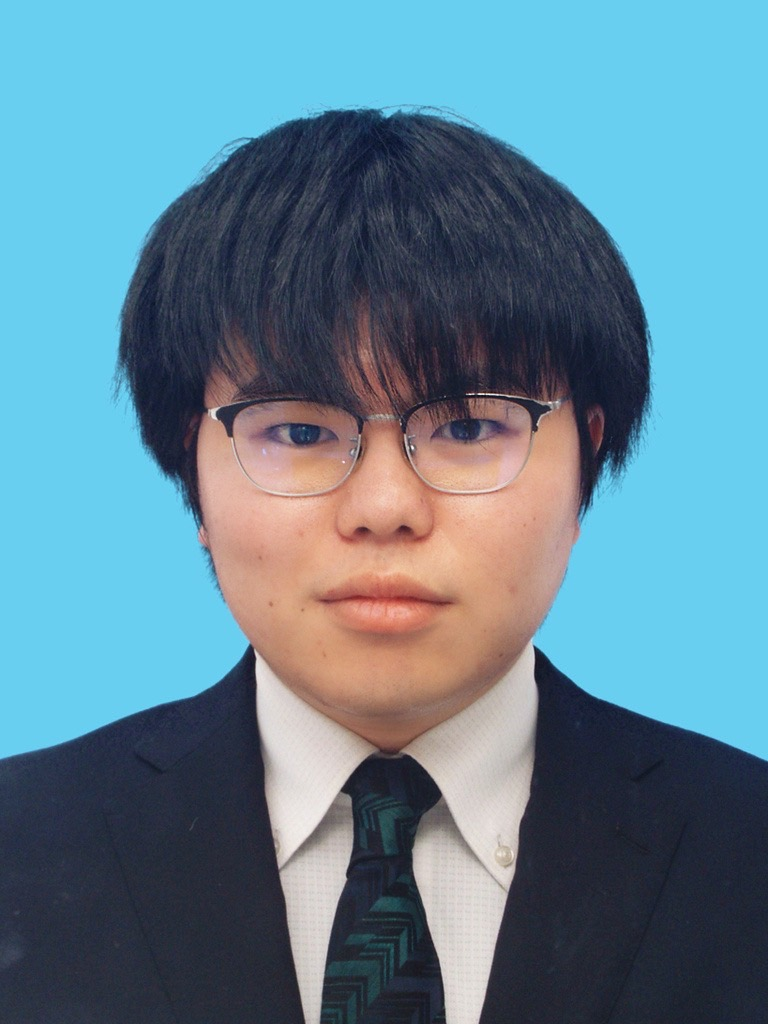
\includegraphics[width=0.3\linewidth]{./fig/profile.jpg}
    \end{minipage}
    \end{tabular}
\end{figure}

\vspace{-1.5em}

\section{About me}
  \vspace{1.0em}
  I am \MyName, a first-year Ph.D.\! student at \OU, Japan, and a specially appointed researcher at SANKEN (The Institute of Scientific and Industrial Research at \OU).
  My research mainly focuses on data stream mining [C1, C2] and causal discovery in time series [C1].
  I am fortunate to be advised by \href{\YSakuraiURL}{\Prof{\YSakurai}} and \href{\YMatsubaraURL}{\Prof{\YMatsubara}} at SANKEN.
  I received my B.Sc.\! and M.Sc.\! degrees from \OU\ advised by \href{\MOnizukaURL}{\Prof{\MOnizuka}} and \href{\YSakuraiURL}{\Prof{\YSakurai}} in March 2023 and 2025, respectively.
  \vspace{0.2em}
  \\
  \textbf{Keywords}:
\smartunderline{Time series analysis}, Data mining, \smartunderline{Stream processing}, \smartunderline{Causality}, Koopman operator theory, Missingness mechanisms, Time series forecasting, \smartunderline{Bayesian optimization}
\vspace{0.2em}
\\
\textbf{Links}:
~\faLinkedin{} \href{https://www.linkedin.com/in/\Linkedin}{Linkedin}
\Separator{}
\faGraduationCap{} \href{https://scholar.google.com/citations?hl=en&user=\Gscholar}{Google Scholar}
\Separator{}
\faGithub{} \href{https://github.com/\GitHubProfile}{GitHub}
\Separator{}
\faOrcid{} \href{https://orcid.org/\ORCID}{ORCID}
\Separator{}
\faTwitter{} \href{https://x.com/\Twitter}{Twitter}
\Separator{}
\faDblp{} \href{https://dblp.org/pid/363/1658.html}{DBLP}
\vspace{0.5em}

\section{\Education}
  \begin{EntriesTableRight}
  \PhD
  \vspace{-0.1em}
  \newline
  \textcolor{gray}{{\fontsize{9pt}{0}\selectfont\PhDDepartment}}
  \vspace{-0.1em}
  \newline
  {\setlength{\leftmargini}{17.2pt}
  \begin{itemize}
  \vspace{-1.0em}
      \item \ExpectedDate
      \item \PhDSupervisor
  \vspace{-1.3em}
  \end{itemize}}
  &
  \hfill
  \Duration{2025}{\Ongoing}
  \vspace{0.30em}
  \newline
  \hfill
  \textcolor{gray}{\fontsize{9pt}{0}\selectfont \texttt{Osaka, \!\!Japan}~}
  \\[4.45em]
  \MSc
  \vspace{-0.1em}
  \newline
  \textcolor{gray}{{\fontsize{9pt}{0}\selectfont\MScDepartment}}
  \vspace{-0.1em}
  \newline
  {\setlength{\leftmargini}{17.2pt}
  \begin{itemize}
  \vspace{-1.0em}
      \item \MScThesis
      \item \MScSupervisor
  \vspace{-1.3em}
  \end{itemize}}
  &
  \hfill
  \Duration{2023}{2025}
  \vspace{0.5em}
  \newline
  \hfill
  \textcolor{gray}{\fontsize{9pt}{0}\selectfont \texttt{Osaka, \!\!Japan}~}
  \\[4.45em]
  \BSc
  \vspace{-0.1em}
  \newline
  \textcolor{gray}{{\fontsize{9pt}{0}\selectfont\BScDepartment}}
  \vspace{-0.1em}
  \newline
  {\setlength{\leftmargini}{17.2pt}
  \begin{itemize}
  \vspace{-1.0em}
      \item \BScThesis
      \item \BScSupervisor
  \vspace{-1.3em}
  \end{itemize}}
  &
  \hfill
  \Duration{2019}{2023}
  \vspace{0.5em}
  \newline
  \hfill
  \textcolor{gray}{\fontsize{9pt}{0}\selectfont \texttt{Osaka, \!\!Japan}~}
\end{EntriesTableRight}


\section{\Experience}
  \begin{EntriesTableRight}
  \textbf{Japan Society for the Promotion of Science (JSPS)}
  \vspace{-0.1em}
  \newline
  \textcolor{gray}{\fontsize{9pt}{0}\selectfont Research Fellow DC1}
  &
  \hfill \Duration{2025}{\Ongoing}
  \vspace{0.25em}
  \newline
  \hfill \textcolor{gray}{\fontsize{9pt}{0}\selectfont \texttt{Osaka, \!\!Japan}~}
  \\
  \textbf{SANKEN}, \OU
  \vspace{-0.1em}
  \newline
  \textcolor{gray}{\fontsize{9pt}{0}\selectfont Specially Appointed Researcher}
  &
  \hfill \Duration{2023}{\Ongoing}
  \vspace{0.25em}
  \newline
  \hfill \textcolor{gray}{\fontsize{9pt}{0}\selectfont \texttt{Osaka, \!\!Japan}~}
  \\
  \textbf{School of Engineering}, \OU
  \vspace{-0.1em}
  \newline
  \textcolor{gray}{\fontsize{9pt}{0}\selectfont Teaching Assistant for ``Exercises in Mathematical Analysis''}
  &
  \hfill \Year{2023}
  \vspace{0.45em}
  \newline
  \hfill \textcolor{gray}{\fontsize{9pt}{0}\selectfont \texttt{Osaka, \!\!Japan}~}
  \\
  \textbf{Graduate School of Information Science and Technology}, \OU
  \vspace{-0.1em}
  \newline
  \textcolor{gray}{\fontsize{9pt}{0}\selectfont Assistant in the detection of variable celestial objects}
  &
  \hfill \Duration{2021}{2023}
  \vspace{0.45em}
  \newline
  \hfill \textcolor{gray}{\fontsize{9pt}{0}\selectfont \texttt{Osaka, \!\!Japan}~}
  \\
  \textbf{Nagase Co., Ltd.}
  \vspace{-0.1em}
  \newline
  \textcolor{gray}{\fontsize{9pt}{0}\selectfont Digital Technology Engineer}
  &
  \hfill \Duration{2020}{2023}
  \vspace{0.45em}
  \newline
  \hfill \textcolor{gray}{\fontsize{9pt}{0}\selectfont \texttt{Tokyo, \!\!Japan}~}
\end{EntriesTableRight}


\section{\Awards}
  \newcommand{\AwardEntry}[4]{%
  \parbox[t]{\linewidth}{{\hypersetup{urlcolor=black} \href{#2}{#1}#4}}
  &
  #3 \\
}

\begin{EntriesTableRight}
  \AwardEntry{\OsakaUnivAward}{}{\Year{Mar \!2025}}{}
  \AwardEntry{\csname DEIM2025Presentation\endcsname}{}{\Year{Mar \!2025}}{}
  \AwardEntry{\textbf{\YamashitaAward}}{https://www.ipsj.or.jp/award/yamasita2024-detail.html\#dbs}{\Year{Jul \!2024}}{}
  \AwardEntry{\csname DEIM2024RunnerUp\endcsname}{https://confit.atlas.jp/guide/event/deim2024/static/awards}{\Year{Jun \!2024}}{ (top 1.4\%)}
  % \AwardEntry{Osaka University Humanware Innovation Program Scholarship}{}{ \Duration{2023}{\Ongoing}}{}
\end{EntriesTableRight}


\section{\Publications}
  \vspace{1.0em}
{\fontsize{12pt}{0}\textbf{\Peerreviewed}}
\begin{EntriesTablePublications}
  % [C3] &
  % \Me, \RFujiwara, \YMatsubara, and \YSakurai.
  % \textbf{Nova: Learning Nonlinear Time-varying Dynamical Systems from Data Streams with Koopman Operator}.
  % (Under submission to AAAI).
  % \\

  [C2] &
  \Me, \RFujiwara, \YMatsubara, and \YSakurai.
  \textbf{CANMI: Causal Discovery under Nonstationary Missingness Mechanisms}.
  (Under submission to NeurIPS).
  \\

[C1] &
  \Me, \YMatsubara, \RFujiwara, and \YSakurai.
  \textbf{Modeling Time-evolving Causality over Data Streams}.
  Proceedings of the 31st ACM SIGKDD Conference on Knowledge Discovery and Data Mining (\textbf{KDD '25}), Toronto, ON, Canada, August 3-7, 2025. Acceptance rate: 19\%. \DOI{10.1145/3690624.3709283}.
  \newline
  \hspace*{-0.12em}
  \GitHub{C-Naoki/ModePlait}
  \Separator{}
  \video{01hS6R1a8jg}
  \\

[W1] &
  \Me, \YMatsubara, \RFujiwara, and \YSakurai.
  \textbf{Stream Mining Time-evolving Causality in Time Series}.
  The 30th ACM SIGKDD Conference on Knowledge Discovery and Data Mining (KDD '24) PhD Consortium, Barcelona, Spain, August 25-29, 2024.
  \URL{kdd2024.kdd.org/ph-d-consortium}.
  \\

[J2] &
  \Me, \YMatsubara, \RFujiwara, and \YSakurai.
  \textbf{Real-time Forecasting of Time-evolving Data Streams using Dynamic Mode Decomposition}.
  IPSJ Transactions on Databases (TOD), Vol. 17, No. 2, pp. 1-11, April 23, 2024. \URL{ipsj.ixsq.nii.ac.jp/records/233825}.
  \\

[J1] &
  \Me, Tadafumi Takata, Yasuhiro Fujiwara, Koki Noda, Keisuke Toyoda, Kaito Higuchi, and \MOnizuka.
  \textbf{Effective detection of variable celestial objects using machine learning-based periodic analysis}.
  Astronomy and Computing, Vol. 45, pp. 100765, November 3, 2023. \DOI{10.1016/j.ascom.2023.100765}.
  \\

\end{EntriesTablePublications}

{\fontsize{12pt}{0}\textbf{\NonPeerreviewed}}

\begin{EntriesTablePublications}
[N4] &
  \Me, \YMatsubara, \RFujiwara, and \YSakurai.
  \textbf{時間変化する因果関係の抽出に基づいた高速将来予測}.
  The 17th Forum on Data Engineering and Information Management (DEIM2025), Fukuoka, Japan, February 27 - March 4, 2025.
  \newline
  \textcolor{mediumred}{\textsb{Student Presentation Award.}}
\\

[N3] &
  \Me, \YMatsubara, \RFujiwara, and \YSakurai.
  \textbf{動的モード分解を活用した高速将来予測アルゴリズム}.
  The 16th Forum on Data Engineering and Information Management (DEIM2024), Hyogo, Japan, February 28 - March 5, 2024.
  \newline
  \textcolor{mediumred}{\textsb{Best Paper Award Runner-up, IPSJ Yamashita SIG Research Award.}}
  \\

[N2] &
  Aiyi Li, Kenya Hoshimure, Kei Tanigaki, Yota Hatano, Reina Nozawa, Yuki Sakamoto, Yuanzhou Wei, \Me, and Naoki Kodani.
  \textbf{Semi-autonomous Leader-follower Approach for Swarm Drone Guidance}.
  The 36th SICE Symposium on Decentralized Autonomous Systems, Tokyo, Japan, February 16-17, 2024.
  \\

[N1] &
  \Me, Tadafumi Takata, Yasuhiro Fujiwara, and \MOnizuka.
  \textbf{周期解析による変動天体の検出}.
  The 15th Forum on Data Engineering and Information Management (DEIM2023), Gifu, Japan, March 5-9, 2023.
\end{EntriesTablePublications}

{\fontsize{12pt}{0}\textbf{\Patents}}

\begin{EntriesTablePublications}
  [P1] & Yasuhiro Fujiwara, \MOnizuka, and \Me.
  \textbf{検出装置、検出⽅法及びプログラム}.
  特開2025-000129, January 7, 2025. \URL{jglobal.jst.go.jp/detail?JGLOBAL\_ID=202503009056531197}.
\end{EntriesTablePublications}


\section{Academic Services}
  \vspace{1.0em}
{\fontsize{11pt}{0}\textbf{External Reviewers}}

\begin{tabular}{cc}
  \begin{minipage}[h]{0.17\textwidth}
    {\setlength{\leftmargini}{17.2pt}
    \begin{itemize}
      \vspace{0.9em}
      \item ACM WWW
      \item ACM SIGKDD
    \end{itemize}}
  \end{minipage} &
  \begin{minipage}[h]{0.83\textwidth}
    {\setlength{\leftmargini}{-5pt}
    \begin{itemize}
      \vspace{0.9em}
      \item[] 2025
      \item[] 2025
    \end{itemize}}
  \end{minipage}
\end{tabular}

\vspace{1.0em}
{\fontsize{11pt}{0}\textbf{Conference Volunteer Work}}

\begin{tabular}{cc}
  \begin{minipage}[h]{0.17\textwidth}
    {\setlength{\leftmargini}{17.2pt}
    \begin{itemize}
      \vspace{0.5em}
      \item PAKDD
      % \item[]
    \end{itemize}}
  \end{minipage} &
  \begin{minipage}[h]{0.83\textwidth}
    {\setlength{\leftmargini}{-5pt}
    \begin{itemize}
      \vspace{0.5em}
      \item[] 2023
      % \item[]
    \end{itemize}}
  \end{minipage}
\end{tabular}


\end{document}
